\section{Evaluation}

This section evaluates the performance of BlueDBM by measuring its latency,
bandwidth and scalability, as well as demonstrating the performance benefits of
simple analytics accelerators doing in-storage computation.

\subsection{Latency}

Figure~\ref{fig:result_latency} shows the access latency of reading data from
various locations in BlueDBM to various locations. It can be seen that when
accessing remote data, the high-speed network helps reduce latency.

\begin{figure}[h]
	\begin{center}
	%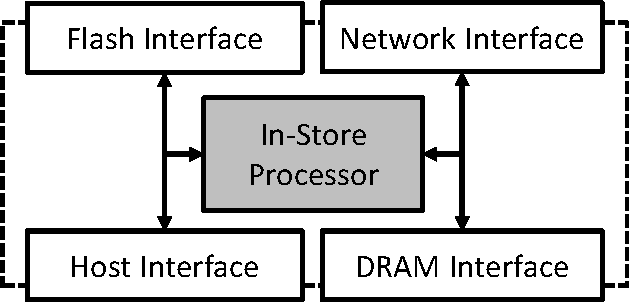
\includegraphics[width=0.3\paperwidth]{figures/isp-service-crop.pdf}
	\caption{Latency of Data Access in BlueDBM}
	\label{fig:result_latency}
	\end{center}
\end{figure}
%Latency for 
%
%fpga<-> flash
%fpga<-> remote flash
%
%host<-> flash
%host<-> remote flash
%host<-> remote host DRAM
%fpga<-> remote ssd using samsung...


\subsection{Bandwidth}

Figure~\ref{fig:result_bandwidth} shows the read bandwidth performance of
BlueDBM while reading over various datapaths. 

\begin{figure}[h]
	\begin{center}
	%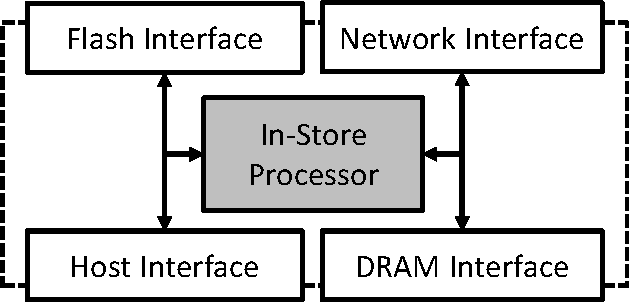
\includegraphics[width=0.3\paperwidth]{figures/isp-service-crop.pdf}
	\caption{Bandwidth of Data Access in BlueDBM}
	\label{fig:result_bandwidth}
	\end{center}
\end{figure}

\subsection{Scalability}

We evaluated the scalability of BlueDBM using a benchmark in which all nodes
competed to read data from all nodes. Figure~\ref{fig:result_scalability} shows
the results of the benchmark. It can be seen that the aggregate bandwidth of all
nodes scale linearly as the number of nodes increase.

\begin{figure}[h]
	\begin{center}
	%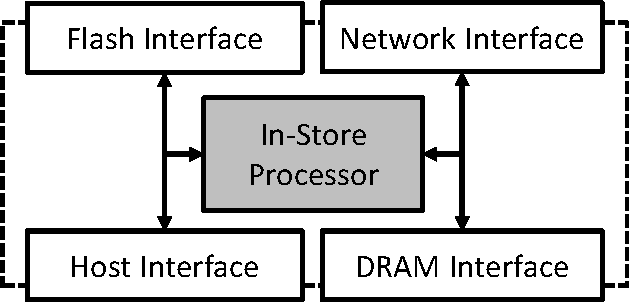
\includegraphics[width=0.3\paperwidth]{figures/isp-service-crop.pdf}
	\caption{Data Access Scalability}
	\label{fig:result_scalability}
	\end{center}
\end{figure}

%Latency for local flash reads, reads from local DRAM, remote reads over
%fpga/serial, remote reads over serial/host DRAM, remote reads over
%ethernet/Flash ethernet/DRAM
%
%Aggregate bandwidth for flash, collecting all flash to one node, flash to pcie?
%
%Aggregate bandwidth for competing workloads on multiple servers, to test
%scalability

\subsection{Performance Benefits in Distributed Analytics}

We evaluated the benefits of BlueDBM in the analytics setting by using the
following synthetic benchmark: Read a 8K 64K 4M block look for number of certain
4-byte value.
We compared scenarios with varying percentage of the data fitting in host DRAM.
(because host DRAM is lower latency than flash. Thankfully, only the counting
results need to come back from the host, circumventing the PCIe bandwidth issue)
(read bandwidth is still important, since we will test SW filtering from flash)

HW/SW filtering while (network: ethernet/aurora/aurora, but as separate
appliance)

\begin{figure}[h]
	\begin{center}
	%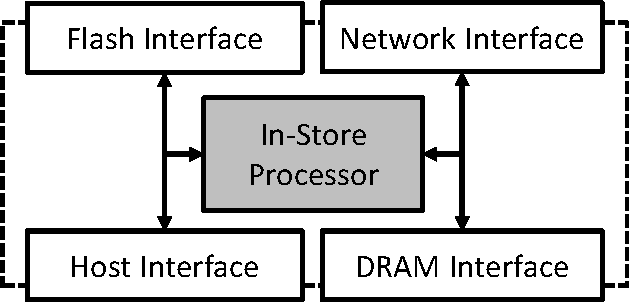
\includegraphics[width=0.3\paperwidth]{figures/isp-service-crop.pdf}
	\caption{Analytics Performance}
	\label{fig:result_analytics}
	\end{center}
\end{figure}
